% Discussion of different hardware techniques
% Aimee, 1 nov 2013

\subsubsection{Virtex FPGA with a Two-Dimensional Reconfiguration Core}
\label{sec:fpga}
On Virtex-4 FPGAs, two-dimensional dynamic reconfiguration like figure \ref{fig:2d} is supported. With 2D reconfiguration it becomes possible to reconfigure device portions whose height is not constrained to be the device height. This architecture of the reconfiguration core (or RC) speeds up the reconfiguration time and thus the evolution time.  The RC can also deploy more candidate solutions as discussed in \cite{virtex4}, which are arrays of bidimensional cell (see figure \ref{fig:candidate}). An alternative for candidate solutions is a mesh-type systolic array of parallel processing elements (PEs) from \cite{dpr}, also following a 2D architecture for the RC. A major feature is the possibility to change the functionality of the PEs by means of Dynamic and Partial Reconfiguration (DPR). This gives the system the capability to adapt. The outputs of the PEs (east and south side) are connected to the close neighbour's input (west and north side), such that only the lowest and right-most PE has to be read for data output. This systolic approach of communication reduces the reconfiguration time and makes the architecture easy to extend.

A drawback of using Virtex FPGAs are the feed-through signales, mentioned in \cite{erlangen}. Each module must be implemented with all possible feed-through channels  needed by other modules. Because we only know at run-time which module needs to feed through a signal, many channels reserved for a possible feed-through become redundant. Also, modules accessing external pins are no longer relocatable, because they are complied for fixed locations where a direct signal line to these pins is established.

% -- Plaatje 2D RC architecture ---------------------------
\begin{figure}[htb]%
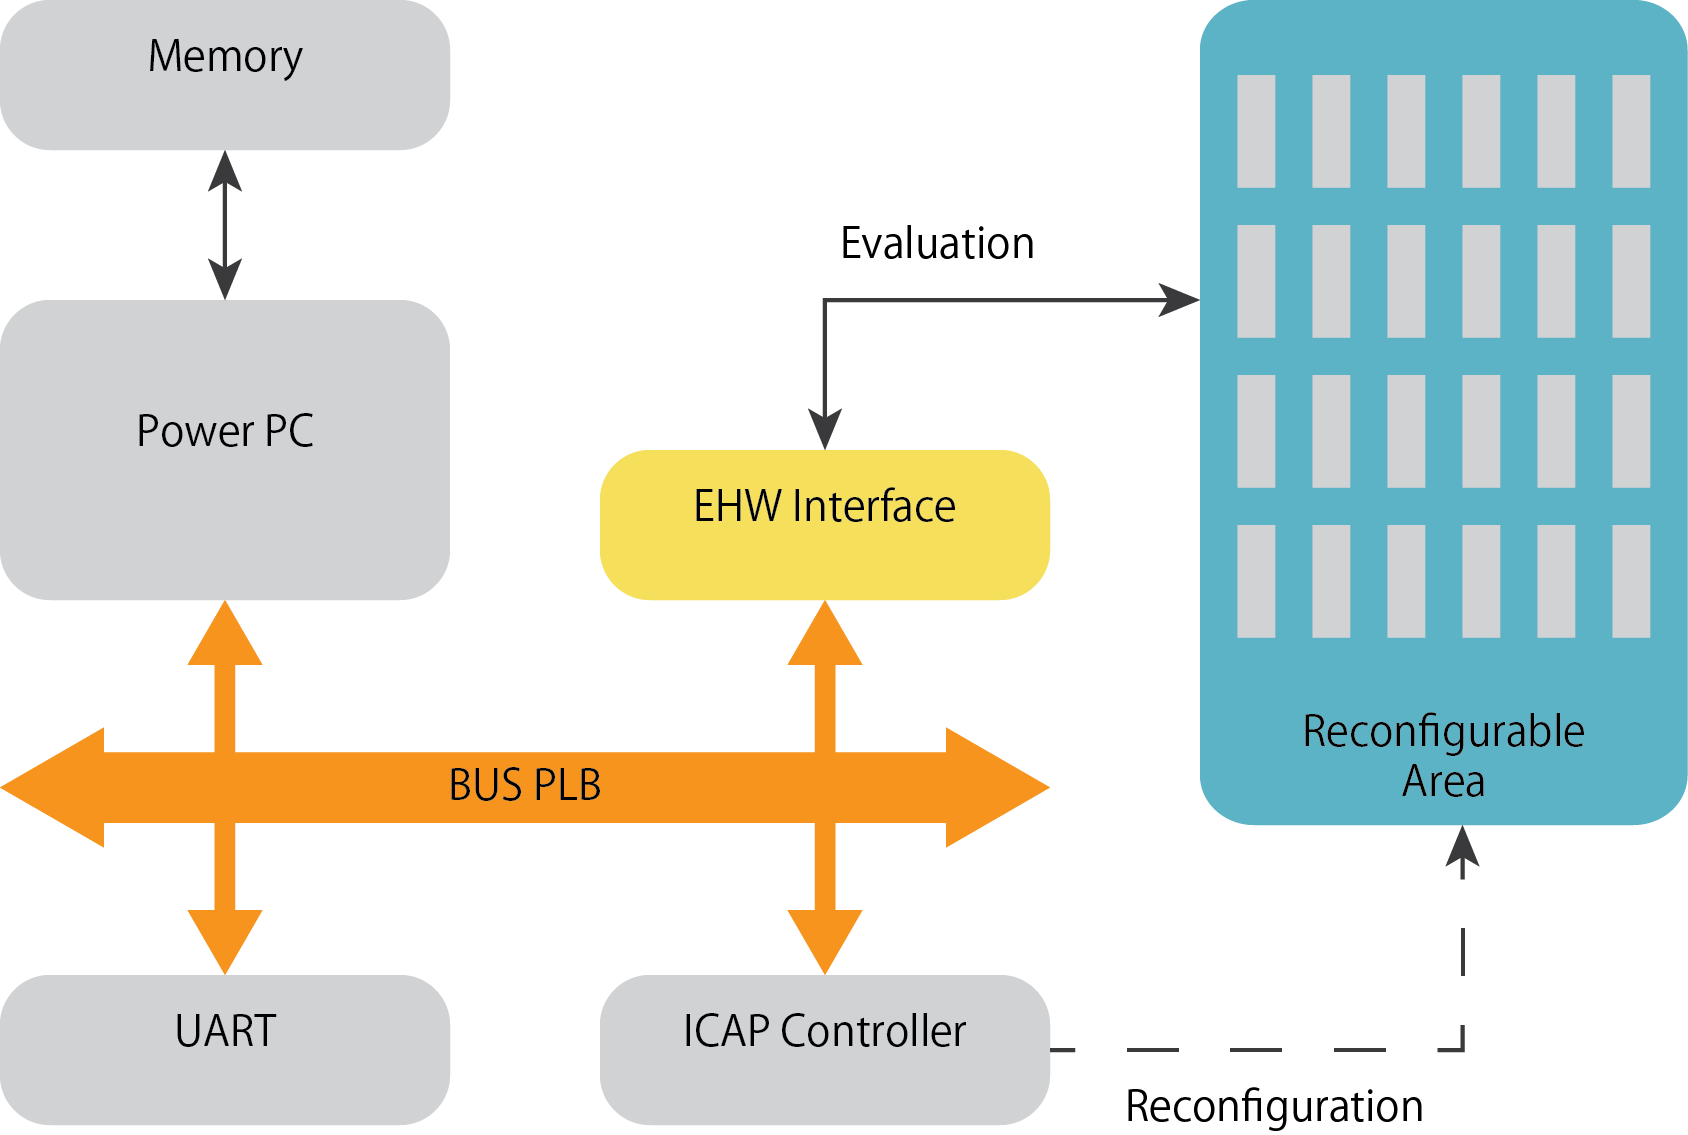
\includegraphics[width=\columnwidth]{Pictures/2D_architecture.png}%
\caption{High-level structure of a Two-Dimensional Architecture depicted in \cite{virtex4}}%
\label{fig:2d}%
\end{figure}

\subsubsection{Candidate Solutions and Direct Bitstream Manipulation}

With a 2D architecture for the RC, \cite{virtex4} uses safe manipulation of the bitstream to overcome the unknown and undocumented bitstream mentioned in \ref{sec:virtex4}. Candidate solutions are used to fill the RC with cells, which have an internal flip-flops allowing the evolution of synchronous circuits. This is a common structure for evolvable hardware (EHW) systems making use of direct bitstream manipulation \cite{virtex4}. For the cell structure of the candidate solutions the use of LUTs and a MUX is proposed, in order to provide direct bitstream manipulation. Combined with the 2D-reconfiguration mechanism, the new architecture causes a speed up of 16x factor. For this system, only Virtex-4 or Virtex-5 FPGAs can be used since Virtex-II does not support 2D reconfiguation (\cite{virtex4}.

% -- Plaatje candidate solutions architecture ---------------------------
\begin{figure}[htb]%
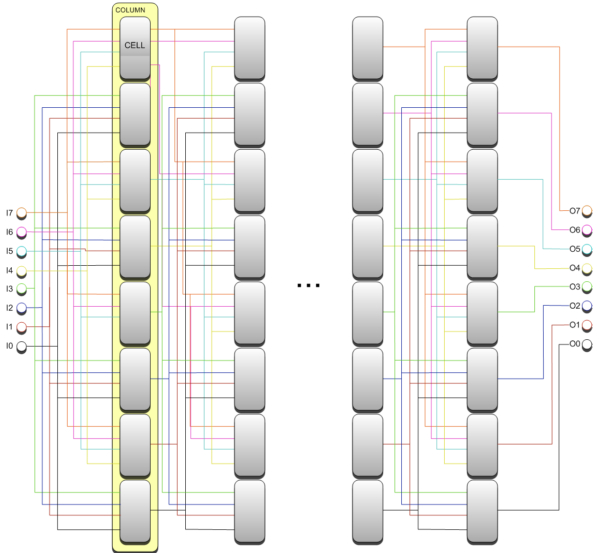
\includegraphics[width=\columnwidth]{Pictures/candidate.png}%
\caption{Internal structure of a Candidate Solution proposed in \cite{virtex4}}}%
\label{fig:candidate}%
\end{figure}

\subsubsection{Systolic array of PEs and Optimized DPR}
\label{sec:dpr}
Other than \cite{virtex4}, \cite{dpr} uses a systolic array of PEs. In this approach, each PE is a basic computation unit able to perform a single operation on the data take from their close neighbors. The architecture can be easily extended to any other processing purposes, since new PEs can be added to the library. In addition, PEs included in this library can be reused among applications. As can be seen in fig. \ref{fig:pe}, the size of the implemented structure is 4x4, but it can be completely and easily scaled. This DPR with elements relocation is carried out using a special HW block, the reconfiguration engine (RE).

\cite{dpr} describes an implementation of this RE. By storing only the body of the bitstream (cutting of the header and the tail), overclocking the FPGA by 2,5x and including internal memory (to avoid pasting the same configuration module in different positions of the architecture) the DPR is optimized. Due to this the reconfiguration time is greatly reduced. Adding the header and the tail of the bitstream at runtime has two additional advantages: it is allowed having a unique bitstream for each PE that can be configured in any position of the array. Also, bitstream reduction reduces the data transference time from the external memory.

% -- Plaatje systolic PE array architecture ---------------------------
\begin{figure}[htb]%
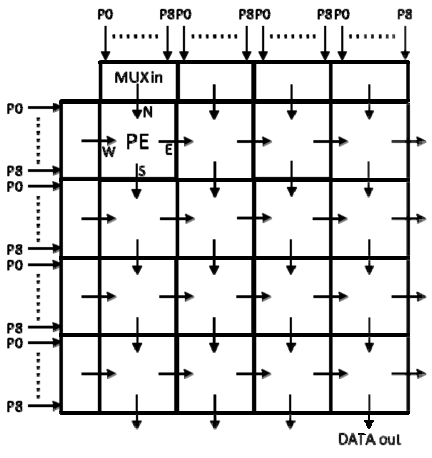
\includegraphics[width=\columnwidth]{Pictures/PE}%
\caption{Systolic array of PEs introduced by \cite{dpr}}%
\label{fig:pe}%
\end{figure}

\subsubsection{Erlangen Slot Machine}
The architecture of \cite{erlangen} the Erlangen Slot Machine (ESM) deals with the three drawbacks of FPGAs mentioned in \ref{sec:fpga}, being fixed pins which are spread around the device (I/O dilemma0, the inter-module dilemma and the local memory dilemma. 

First, the I/O dilemma caused by fixed pins spread around the device is solved by connecting all bottom pins from the FPGA to an interface controller realizing a crossbar, as can be seen in figure \ref{fig:erlangen}. It connects FPGA pins to peripherals automatically based on the slot position of a placed module. This I/O rerouting principle is done without reconfiguration of the crossbar FPGA.

Second, the memory dilemma has been solved. In normal Virtex-II FPGAs, a module can only occupy the memory inside its physical slot boundary. Storing data in off-chip memories is therefore the only solution. In the ESM, six SRAM banks are connected to the FPGA. Since these banks are placed at the opposite side as the crossbar, a module will connect to peripherals from one side, while the other side will be used for temporally storing computational data. In order to use a SRAM bank (called a slot), the module must have at least a width of three micro-slots, in which the total device is divided (see \ref{fig:erlangen}). This organization simplifies relocation, enabling a partially reconfigurable computing system. Also, equal resources will be available for each module.

Finally, the inter-module communication dilemma is dealt with. Dynamically routing signal lines on the hardware is a very difficult task. The ESM uses a combination of bus-macros, shared memory, RMB (Reconfigurable Multiple Bus) and a crossbar to take away the limiting factor for the wide use of partial dynamic reconfiguration (\cite{erlangen}).

% -- Plaatje ESM ---------------------------

\begin{figure}[htb]%
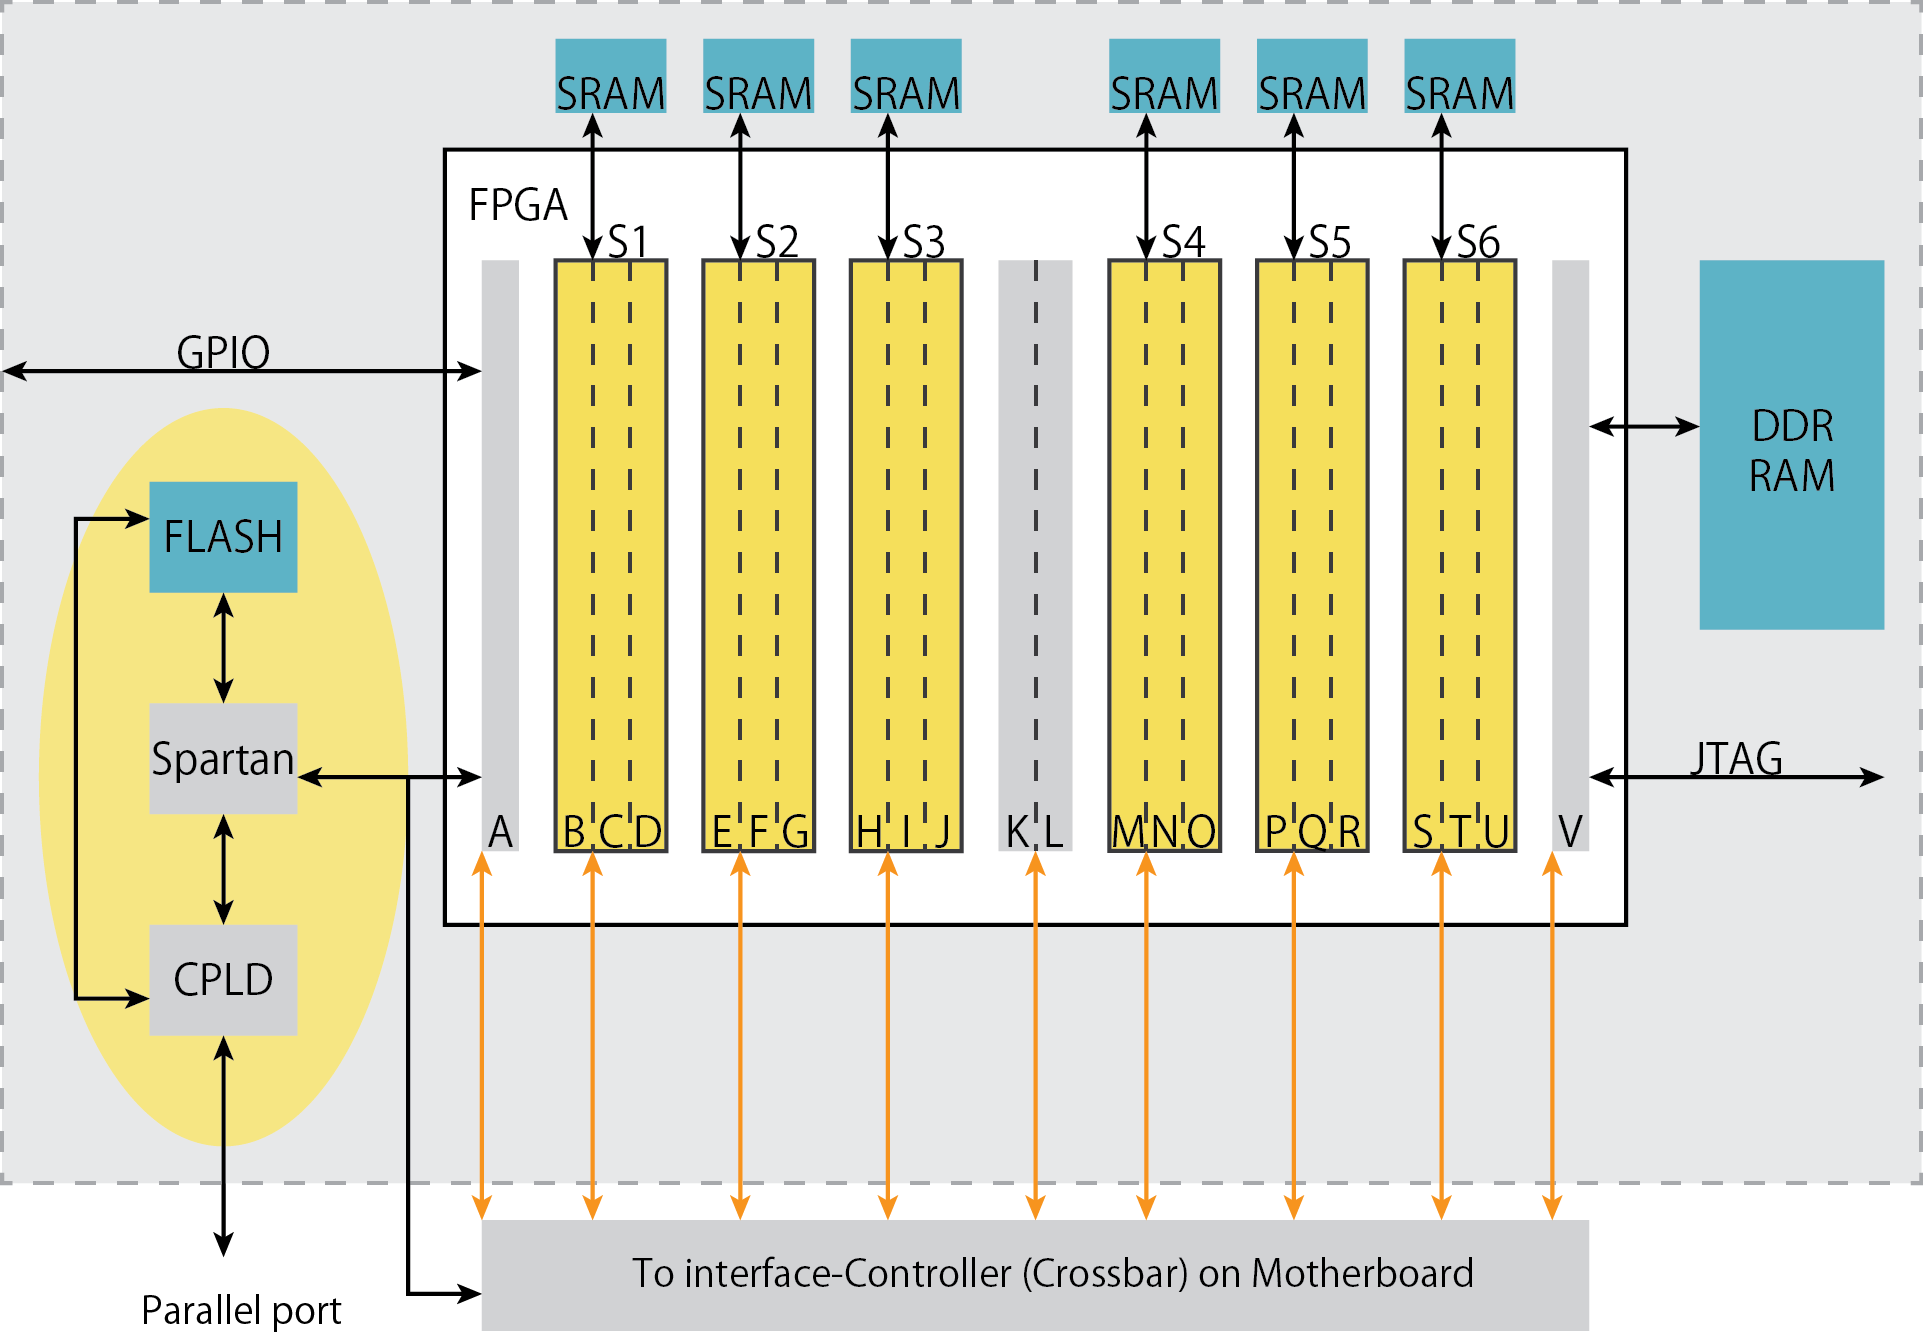
\includegraphics[width=\columnwidth]{Pictures/erlangen}%
\caption{Architecture of the ESM board. Three consecutive micro-slots define a macro-slot, which can access one full external SRAM bank.}%
\label{fig:erlangen}%
\end{figure}
